\newpage
\pagebreak
\section{Ejercicio 5}
\subsection{Problema}
Una vez elegidos los mejores valores de configuraci\'on para cada heur\'istica implementada (si fu\'e posible), realizar una \textbf{experimentaci\'on sobre un conjunto nuevo de instancias}  para observar la performance de los m\'etodos comparando nuevamente la calidad de las soluciones obtenidas y los tiempos de ejecuci\'on en funci\'on del tama\~no de entrada. Para los casos que sea posible, comparar tambi\'en los resultados del algoritmo exacto implementado. Presentar todos los resultados obtenidos mediante gr\'aficos adecuados y discutir al respecto de los mismos.
\subsection{Explicaci\'on del problema}

Como los anteriores cuatro ejercicios trabajamos con la misma familia de arboles, buscamos distintas variantes para ver si nuestras heuristicas tiene alguna caracteristica particular segun el tipo de grafo donde la estemos ejecutando. Como vimos anteriormente, para una familia de grafos Kn, la H1 suele tardar menos que la H2 sin embargo la segunda suele conseguir mejores resultados. Ademas vimos que nuestra variante H3 se situa en un punto medio cuando tenemos muchos colores. Cuando tenemos pocos, las tres heuristicas suelen tardar lo mismo. \\
Analizaremos en esta seccion como se comportan los grafos Estrella/Arboles (grafos bipartitos) y que sucede a medida que agregamos aristas a medida que llegamos a obtener nuestro Kn. 
\subsection{Tests y Performance}
Vamos a empezar con un grafo estrella y paso a paso agregaremos 1 arista hasta llegar a un Kn. Lo primero que veremos es que Los grafos estrella se comportan bastante parecidos en relacion a los Kn. vemos en el siguiente grafico que a medida que vamos transformando una estrella en un Kn, el tiempo aumenta de la misma manera.
\pagebreak

\begin{figure}[h!]
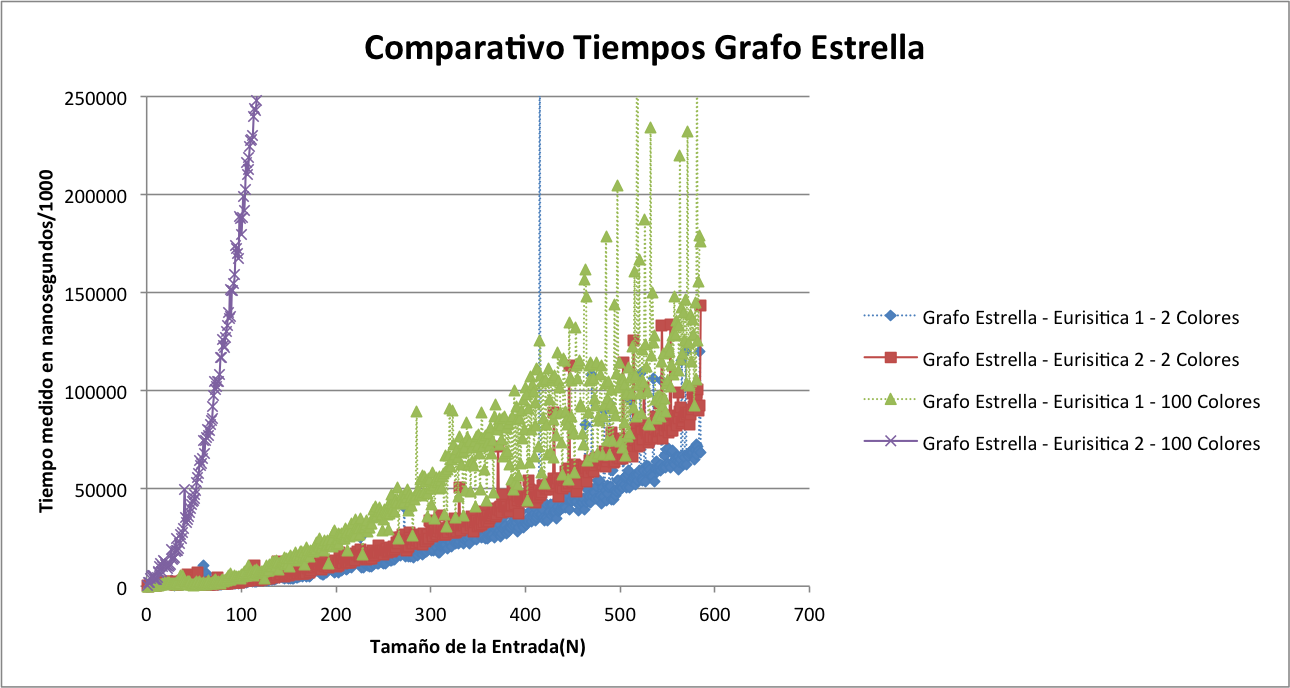
\includegraphics[width=140mm]{ejercicio4/ej5-estrella.png}
\centering
\caption{Cantidad de conflicos HFINAL por solucion}
\label{overflow3}
\end{figure}



Otra cosa que veremos sera como se comporta nuestra solucion de backtrack en comparacion a la "heuristica final". Esta heuristica se basa en nuestro analisis anterior. Miraremos el 20$\%$ de las materias aleatoriamente y si todas tienen mas de 20 colores( es decir que tenemos muchos colores) entonces usaremos la H3. Caso contrario usaremos la H2.


\begin{figure}[h!]
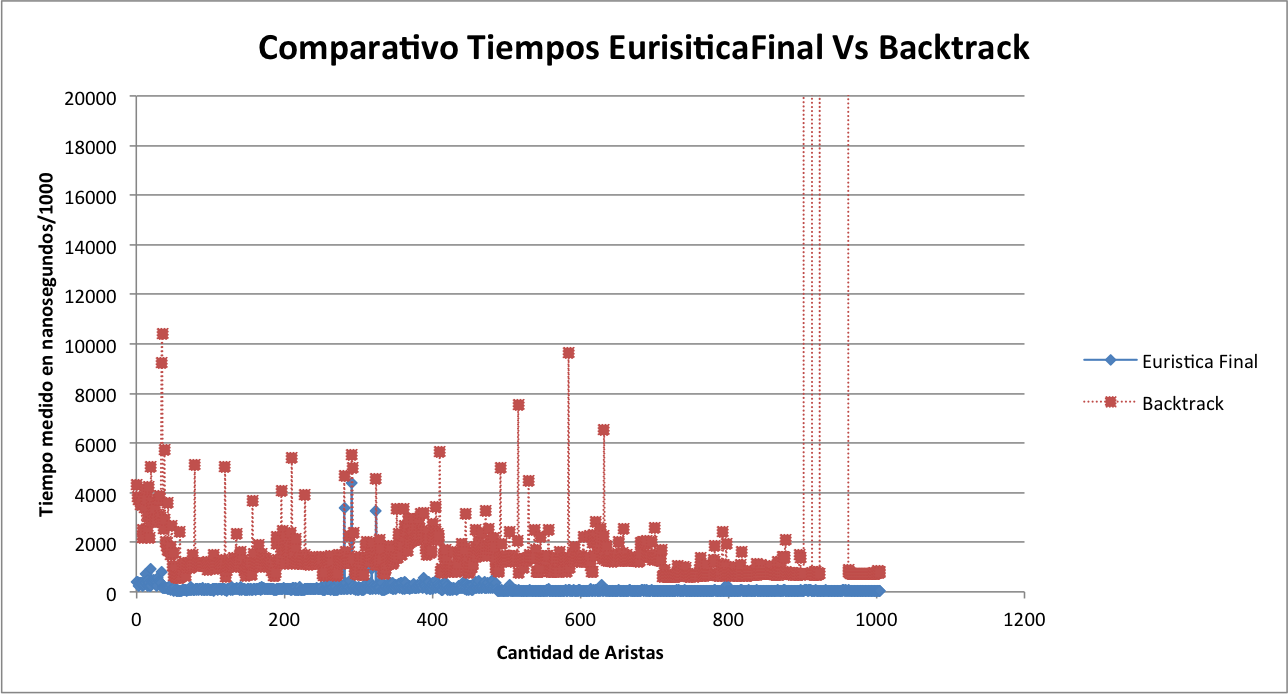
\includegraphics[width=140mm]{ejercicio4/ej5-tiempo-hf-backtrack.png}
\centering
\caption{Comparacion Tiempos estrella HFINAL vs BACKTRACK CON PODAS}
\label{overflow3}
\end{figure}

\pagebreak

En este caso la heuristica final elijio la H2 y lo que muestra el grafico es que si bien el backtrack te asegura la solucion optima, la heruistica final nos dio una cantidad relativamente baja de conflictos y el tiempo se situa extremadamente por debajo. De todos los casos analizados, tuvo el 18,8$\%$ conflictos y ninguno de esos casos tuvo mas de un conflicto. Este porcentaje sale de ver el siguiente grafico: 

\begin{figure}[h!]
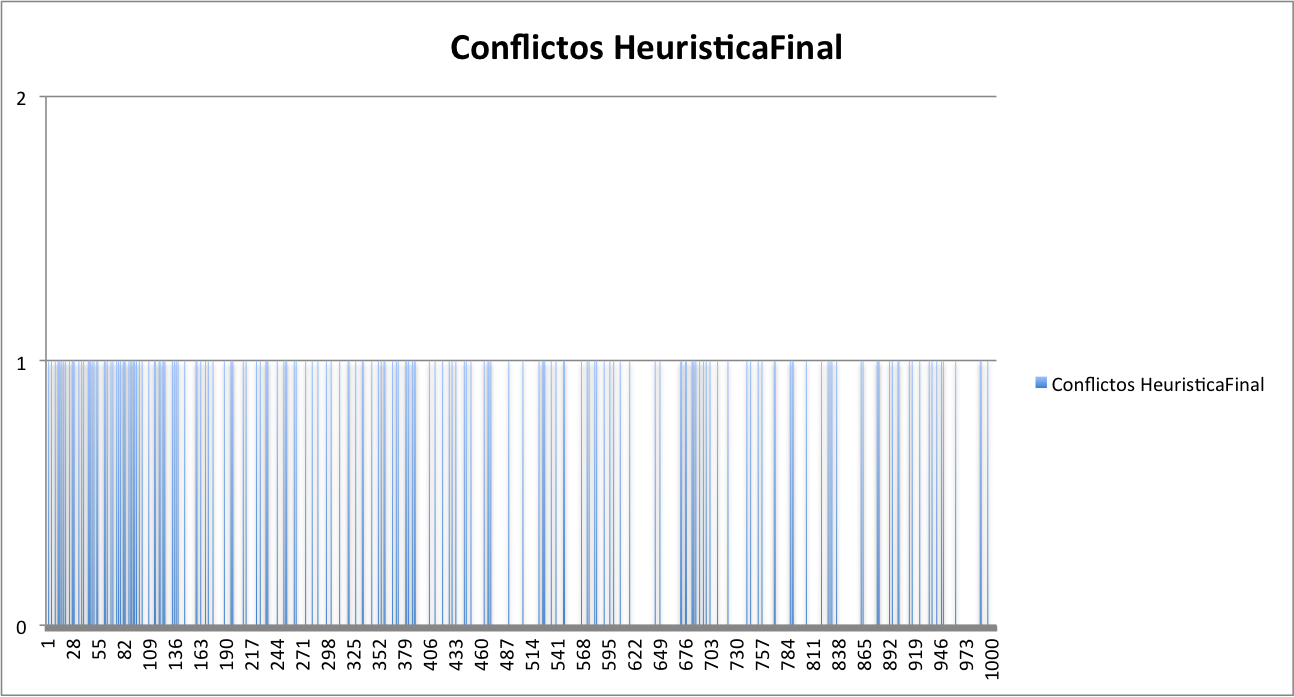
\includegraphics[width=140mm]{ejercicio4/ej5-conflictos.png}
\centering
\caption{Cantidad de conflicos HFINAL por solucion}
\label{overflow3}
\end{figure}
\\
\\
Por ende, si uno prefiere optimalidad, tendra que pagar el costo de corer un algoritmo exacto mientras que si uno tiene un margen de error no tan grande, puede correr una solucion polinomial y tener un resultado aproximado.

Luego decidimos seguir experimentando con nuevas familias de grafos y analizamos los grafos bipartitos completos. Para este realimos nuevos generadores, y nuevos tests para mostrar la diferencia de tiempos entre nuestra mejor euristica y un algoritmo exacto como backtrack.


En el siguiente grafico vemos la comparaci\'on de lo que estabamos proponiendo, y lo que no se observa en el grafico es que los dos algoritmos encuentran una soluci\'on optima sin conflictos.

\begin{figure}[h!]
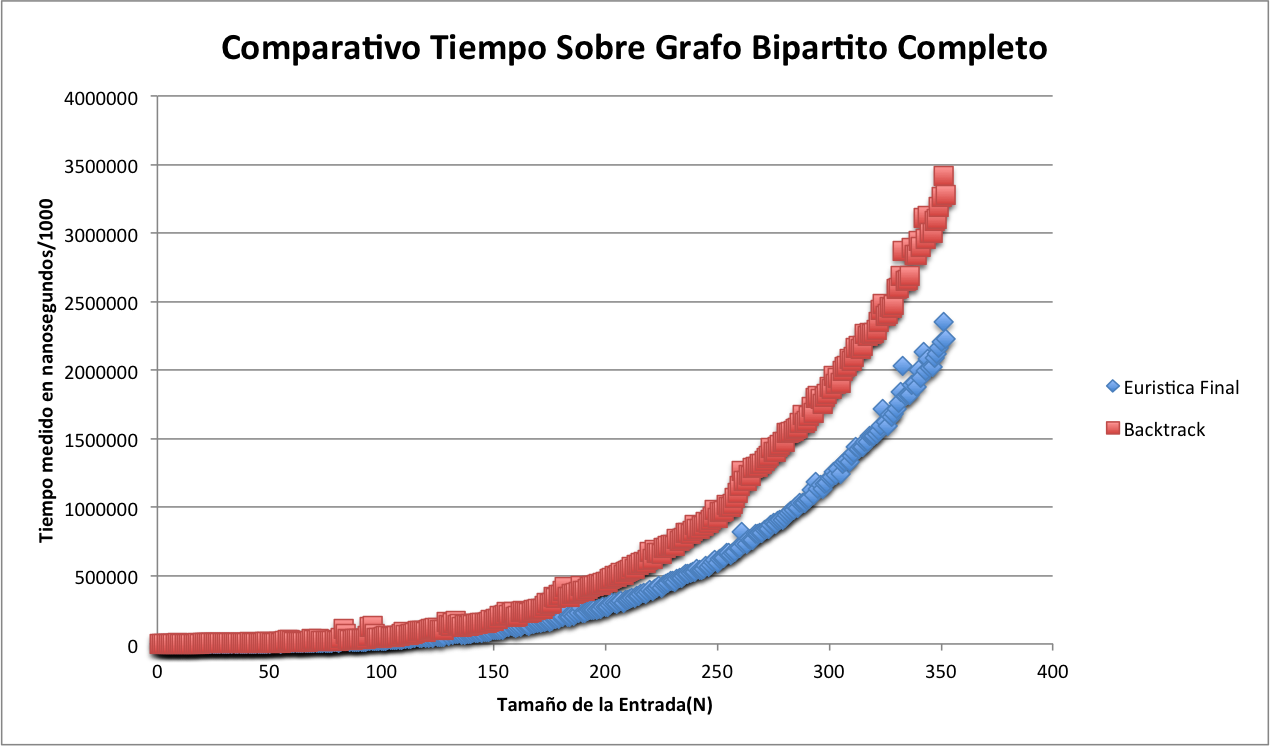
\includegraphics[width=140mm]{ejercicio4/ej5-bipartitoCompleto.png}
\centering
\caption{Cantidad de conflicos HFINAL por solucion}
\label{overflow3}
\end{figure}

Como veniamos probando con muchos grafos estructurados, decidimos empezar a conectar grafos aleatoriamente, intentando evitar familias de grafos conocidas.
Comenzando con 100 nodos desconectados, 8 colores por nodo, fuimos conectando de a 100 aristas en un orden random, para ver como se comportaban los algoritmos. Este test lo podemos plasmar en la siguiente tabla:


\begin{tabular}{| l | l | c | r |}
  \hline
Cantidad aristas & Tiempo Heurisitca & Conflictos Heuristica& Tiempo Backtrack \\ \hline
100 &1133.879 & 36 & 6526.428   \\ \hline
200 &1583.267 & 24 & 8010.119   \\ \hline
300 &1507.946 & 26 & 5874.094   \\ \hline
400 &1770.348 & 21 & 6543.094   \\ \hline
500 &1824.115 & 24 & 5348.103   \\ \hline
600 &2173.457 & 14 & 6424.84   \\ \hline
700 &1397.809 & 19 & 5623.086  \\ \hline
800 &2534.807 & 11 & Tiempo No Medible   \\ \hline
\end{tabular}

\pagebreak